A formal definition of a machine learning algorithm is given by \cite{Mitchell:1997:ML:541177}: "A computer program is said to learn from experience $E$ with respect to some class of tasks $T$ and performance measure $P$ if its performance at tasks in $T$, as measured by $P$, improves with experience $E$." 
From such a vague definition, it is obvious that a comprehensive introduction to machine learning is a broad topic. Hence, in this thesis a brief introduction to the \textit{image classification} problem is provided only. That should be enough for a non-expert to be able to read and to understand this whole thesis.

As explained in Section \ref{motivation}, image classification is the \textit{task} of assigning a \textit{label} or a \textit{class} to an image. If an input is an $n$-dimensional vector and there are $k$ classes, then the learning algorithm is usually asked to produce a function $f: \mathbb{R}^n \rightarrow \{1, ... , k\}$. One other variant of a classification task would be to produce a function $f$ which outputs a probability distribution over classes, i.e. how likely each class is. In such a scenario, the next step usually is to assign a label according to the most likely class, but this need not to be the case. A model that is used for classification is called a \textit{classifier}.

After defining a task, it is important to know how to measure the performance of a model. Depending on the domain of a system, this measure can vary. The \textit{accuracy} of the model is usually measured for a classification task. It is the fraction of correct predictions of the model. For example, if the prediction of the model was correct for 8 out of 10 samples, the accuracy of that model (on those 10 samples) is $0.8$ or $80\%$. An equivalent information can be obtained by measuring the \textit{error rate}. It is defined as the fraction of incorrect predictions of the model. 

Usually we are interested how good the model is on previously unseen data, because that way we can see how well will it work in the real world application. Therefore, we measure its performance on a set of data that is not used during training. Such a set of data is called \textit{test set}. A test set is subset of an entire \textit{dataset}.

A dataset is a collection of samples. One of the oldest datasets used in Machine Learning is the Iris flower dataset \cite{iris-dataset}. That dataset consists of 50 samples from each of three species of Iris. For each sample, four measures are taken: the length and the width of the sepals and petals, in centimeters. A measurable property of a sample is called a \textit{feature}. Hence, Iris dataset has 3 classes, 150 samples and each sample has 4 features. A classifier for that dataset could be modelled as a function $f: \mathbb{R}^4 \rightarrow \{0, 1, 2\}$ where $0, 1, 2$  encode the first, the second and the third type of Iris, respectively.

For every sample in a dataset, information is provided that defines what a class of that sample is. That information is called \textit{ground-truth label}. It is usually used as a vector. Assume there are $N$ different classes in a dataset. Then every class can be indexed from $0$ to $N-1$. Let there be a sample such that its ground-truth label has the index $p$. Then a ground-truth vector $\pmb 1_p$ represents a vector with dimensionality $N$ and all the values are $0$, except for the index $p$ where the value is $1$. In other words, a vector $\pmb 1_p$ encodes a ground-truth label.

Most machine learning algorithms have \textit{hyperparameters}, settings that we can use to control the algorithms' behaviour. Hyperparameters are values which are set before the learning algorithm begins. In contrast, the values of other parameters are derived via training. 

If a classifier has a high accuracy on a test dataset, we say it \textit{generalizes} well. However, if it has a high accuracy on the training samples, but a low accuracy on a test dataset, we say it \textit{overfits}. To avoid overfitting, training samples are split into two non overlapping subsets: the \textit{training} subset and the \textit{validation} subset.

The validation subset can be used to find good hyperparameters. The training subset is used to adjust parameters of a model. The validation subset is verifying that any increase in accuracy over the training dataset actually yields an increase in accuracy over a dataset that has not been shown to the model before, or at least the model hasn't been trained on it. If the accuracy over the training dataset increases, but the accuracy over the validation dataset stays the same or decreases, then a model is overfitting. The test accuracy, an accuracy we are typically interested in, is computed on the test dataset. That means that an original dataset is split into three disjoint subsets: training, validation and test subset. 

A problem can occur if there is not enough data, i.e. an original dataset is too small. That makes the training, the validation and the test subset not big enough. For instance, it can happen that the training dataset doesn't have any instances of some specific class or there are too few of them. That problem can be solved by the \textit{k-fold cross-validation} procedure.

That procedure is based on the idea of repeating the training and testing computation on different splits of the original dataset. The original set is split into $k$ equal disjoint subsets. Of the $k$ subsets, a single subset is retained as the validation set for testing the model, and the remaining $k-1$ subsets are used as training data. The process is then repeated $k$ times, with each of the $k$ subsets used exactly once as the validation data. The $k$ results can then be averaged to determine the test accuracy. 

So far, the basics of the machine learning are covered. A goal for the rest of this chapter is to provide a brief introduction to the deep learning area. In Section \ref{subsection:FNN} an introduction to basic neural networks is provided. After that, in Section \ref{subsection:gradient-descent} the Gradient Descent algorithm and variations of it are introduced. Gradient descent is used for optimization of functions based on the derivations of them. The backpropagation algorithm, an efficient algorithm to compute a derivation of a function represented by a neural network, is introduced in Section \ref{subsection:backpropagation}. Finally, in Section \ref{subsection:convolutionalNN} convolutional neural networks are presented. A convolutional neural network represents a typical choice of architecture of the neural network when it comes to the computer vision domain.

\section{Feedforward neural networks}
\label{subsection:FNN}
\textit{Feedforward neural networks} or \textit{multilayer peceptrons} (MLPs) are the essential deep learning models. A feedforward neural network defines a mapping $f (\pmb{x} ; \pmb{\theta}) = \pmb{y}$ and learns the value of the parameters $\pmb{\theta}$ that result in the best function approximation.

A neural network consists of several \textit{layers}. There is always one \textit{input} layer, followed by one or more \textit{hidden} layers and finally, there is an \textit{output layer}. The number of layers (without an input layer) defines a \textit{depth} of the model. There is no precise definition, but neural networks with more than three layers are called \textit{deep} neural networks. 

When it comes to feedforward neural networks, a network is a directed acyclic graph. Vertices of such a graph are called \textit{units} or \textit{neurons} and edges are called \textit{weights}. Vertices represent scalar functions of an input. Weights are the parameters $\pmb \theta$ which a neural network learns. Edges define data flow. One example of such a model is shown in the Figure \ref{fig:basic-cnn}.

\begin{figure}
\begin{tikzpicture}[
plain/.style={
  draw=none,
  fill=none,
  },
net/.style={
  matrix of nodes,
  nodes={
    draw,
    circle,
    inner sep=10pt
    },
  nodes in empty cells,
  column sep=2cm,
  row sep=-9pt
  },
>=latex
]
\matrix[net] (mat)
{
|[plain]| \parbox{1.3cm}{\centering Input\\layer} & |[plain]| \parbox{1.3cm}{\centering Hidden\\layer} & |[plain]| \parbox{1.3cm}{\centering Output\\layer} \\
& |[plain]| \\
|[plain]| & \\
& |[plain]| \\
  |[plain]| & |[plain]| \\
& & \\
  |[plain]| & |[plain]| \\
& |[plain]| \\
  |[plain]| & \\
& |[plain]| \\    };
\foreach \ai [count=\mi ]in {2,4,...,10}
  \draw[<-] (mat-\ai-1) -- node[above] {Input \mi} +(-2cm,0);
\foreach \ai in {2,4,...,10}
{\foreach \aii in {3,6,9}
  \draw[->] (mat-\ai-1) -- (mat-\aii-2);
}
\foreach \ai in {3,6,9}
  \draw[->] (mat-\ai-2) -- (mat-6-3);
\draw[->] (mat-6-3) -- node[above] {Ouput} +(2cm,0);
\end{tikzpicture}

\caption{An example of the feedforward neural network architecture}
\label{fig:basic-cnn}
\end{figure}

A typical architecture of one neuron can be seen in the Figure \ref{fig:basic-neuron}. That specific neuron performs an operation $ f(net) = y $ where $net = x1*w1 + x2*w2 + x3*w3 + bias$.  Bias is usually modelled as an additional input with the corresponding weight $w=1$. Then a neuron performs the operation $ f(\pmb x \times \pmb w) = y$ where $\times$ denotes cross-product between two vectors. Function $f$ is called an \textit{activation function} and usually is the same for all neurons in the same layer. In the input layer the activation function is mapping from input to output, i.e. $f(x) = x$, but in the other layers those are usually non-linear functions. 

 \textit{Convolutional Neural Networks} (CNNs), which are described in Subsection \ref{subsection:convolutionalNN}, are a specific kind of feedforward neural networks. They are most popular in the computer vision domain. If there are cycles in a graph, we are probably talking about the \textit{Recurrent Neural Networks} (RNNs) which are used in domains where a context is important, for instance in Natural Language Processing. However, RNNs are out of the scope of this thesis and will not be further discussed.

\begin{figure}
\begin{tikzpicture}[
init/.style={
  draw,
  circle,
  inner sep=2pt,
  font=\Huge,
  join = by -latex
},
squa/.style={
  draw,
  inner sep=2pt,
  font=\Large,
  join = by -latex
},
start chain=2,node distance=13mm
]
\node[on chain=2] 
  (x2) {$x_2$};
\node[on chain=2,join=by o-latex] 
  {$w_2$};
\node[on chain=2,init] (sigma) 
  {$\displaystyle\Sigma$};
\node[on chain=2,squa,label=above:{\parbox{2cm}{\centering Activation \\ function}}]   
  {$f$};
\node[on chain=2,label=above:Output,join=by -latex] 
  {$y$};
\begin{scope}[start chain=1]
\node[on chain=1] at (0,1.5cm) 
  (x1) {$x_1$};
\node[on chain=1,join=by o-latex] 
  (w1) {$w_1$};
\end{scope}
\begin{scope}[start chain=3]
\node[on chain=3] at (0,-1.5cm) 
  (x3) {$x_3$};
\node[on chain=3,label=below:Weights,join=by o-latex] 
  (w3) {$w_3$};
\end{scope}
\node[label=above:\parbox{2cm}{\centering Bias \\ $b$}] at (sigma|-w1) (b) {};

\draw[-latex] (w1) -- (sigma);
\draw[-latex] (w3) -- (sigma);
\draw[o-latex] (b) -- (sigma);

\draw[decorate,decoration={brace,mirror}] (x1.north west) -- node[left=10pt] {Inputs} (x3.south west);
\end{tikzpicture}
\caption{A single processing unit in a neural network}
\label{fig:basic-neuron}
\end{figure}

\section{Gradient descent}
\label{subsection:gradient-descent}
The accuracy of a parametric model depends on the data provided to train it and the parameters used. The same holds for neural networks. The parameters in the neural networks are weights and during the training we are trying to find \textit{the best} weights. To find them, we express how bad the model is using the \textit{loss function} or \textit{cost function}. It expresses how wrong the model is (for a given data) using the given weights. When such a function is defined, all we do is try to find an input to that function, i.e. weights, such that output of that function, i.e. loss, is minimal. Most machine learning algorithms have some kind of optimization built in. Optimization refers to the task of find $\pmb x$ s.t. $f(\pmb x)$ is maximal or minimal. In this thesis, optimization will always mean minimization, except when stated otherwise. Maximization can be accomplished by minimizing the function $-f(\pmb x)$.

Since training a neural network is actually minimizing a loss function that is represented by the neural network, two things need to be decided: the loss function that will be used and the optimization algorithm that will be used to find its minimum.

The most popular classification loss function is \textit{cross-entropy}. Given two probability mass functions (a mass function is a function that gives the probability that a discrete random variable is exactly equal to some value) $\pmb u$ and $\pmb v$ in $\mathbb{R}^T$, i.e. $\pmb u = (u_1, ..., u_T)$ and $\pmb v =  (v_1, ..., v_T)$, the cross-entropy between $\pmb u$ and $\pmb v$ is
 \begin{equation}
H (\pmb u, \pmb v)= - \sum_{t=1}^T  u_t  \text{ln} v_t 
\end{equation}

Let $\pmb u$ enocde the ground-truth label, $u_c = 1$ where $c$ is index of the class. Let $\pmb v$ be the predicted softmax class scores. Now $H$ measures how dissimilar true and predicted probabilities are for a single sample.

Let $\mathcal{D}$ be a dataset such that
$ \mathcal{D} = \{ (\pmb x_s, \pmb w_s)\}_{s=1}^{S}$ where $x_s$ is an input vector and $w_s$ is a vector encoding the ground truth (i.e. all indices have value $0$, except on the index of the class which $x_s$ represents where the value is $1$).

On this basis, \textit{cross-entropy loss} on $\mathcal{D}$ is defined as
\begin{equation} \label{eq:loss-function}
L(\pmb \theta) = \frac{1}{S} \sum_{s=1}^{S} H (\pmb w_s, \text{softmax} (f(\pmb x_s ; \pmb \theta)))
\end{equation}

Models trained with this loss function are called \textit{softmax classifiers}. If $T = 2$, it is also called \textit{logistic regression}. Classifiers learn to predict probabilities per class label.

After we defined the loss function $L(\pmb \theta)$  as in \ref{eq:loss-function}, we need to find an optimization algorithm to find its minimum. Since the function is not linear in $\pmb \theta$, a nonlinear optimization algorithm is needed. A popular choice in deep learning is \textit{Gradient Descent}.

Gradient Descent is an iterative optimization algorithm that is used for finding the minimum of a function. It is based on the first derivative of the function whose minimum needs to be found. This means that the function must be differentiable. 

Let $\nabla f$ be a vector of all partial derivatives of a function $f: \mathbb{R}^N \mapsto \mathbb{R}^N$. Then $\nabla f(\pmb x) = (f_{x_1}(\pmb x), ..., f_{x_n}(\pmb x))$  encodes how fast $f$ changes with all arguments $x_1, ..., x_n$, which is exactly what is needed for optimizing $L(\pmb \theta)$. Compute the direction of the greatest increase, i.e. $\nabla L(\pmb \theta)$, and move in the opposite direction. The size of that move is called \textit{step size} and it is defined by the \textit{learning rate} - hyperparameter $\alpha$.  

The pseudo code for gradient descent is presented in Algorithm \ref{alg:gradient-descent}.

\begin{algorithm}[htb]
\caption{Gradient Descent}
\label{alg:gradient-descent}

\KwIn{$\pmb \theta, L, \alpha $}

\While {$true$}{
    $\pmb \theta^{'} \leftarrow \nabla L(\pmb \theta)$\;
    \If {$\| \pmb \theta^{'}\|  \approx 0 $} {
    		\Return\;
    }
    $\pmb \theta \leftarrow \pmb \theta - \alpha * \pmb \theta^{'}$\;
}
\end{algorithm}

This algorithm is simple and efficient. Simple since the only requirement is that $f$ is differentiable and efficient because it requires only first derivatives. A problem that can occur is that $\| \pmb \theta^{'}\|  \approx 0$ can happen at all critical points - minimum, maximum and saddle points.

To speed up convergence, \textit{momentum} is introduced using hyperparameter $\beta$. It increases step size dynamically by using $velocity$ $\pmb v$. Velocity builds up momentum if successive gradients are similar. The pseudo code for gradient descent with momentum is shown in Algorithm \ref{alg:gradient-descent-momentum}

\begin{algorithm}[htb]
\caption{Gradient Descent with momentum}
\label{alg:gradient-descent-momentum}

\KwIn{$\pmb \theta, L, \alpha, \beta $}

$\pmb v \leftarrow \pmb 0$\;
\While {$true$}{
    $\pmb \theta^{'} \leftarrow \nabla L(\pmb \theta)$\;
    \If {$\| \pmb \theta^{'}\|  \approx 0 $} {
    		\Return\;
    }
    $\pmb v \leftarrow  \beta \pmb v - \alpha * \pmb \theta^{'}$\;
    $\pmb \theta \leftarrow \pmb \theta + \pmb v$\;
}
\end{algorithm}

The idea behind gradient descent with \textit{Nesterov Momentum}, which works often better than standard Gradient Descent with momentum, is not to evaluate the gradient at the current point, but at the point which would be the next, i.e. evaluate the gradient at $\pmb \theta + \pmb v$ instead of at $\pmb \theta$. The pseudo code is shown in Algorithm \ref{alg:gradient-descent-nesterov-momentum}

\begin{algorithm}[htb]
\caption{Gradient Descent with Nesterov momentum}
\label{alg:gradient-descent-nesterov-momentum}

\KwIn{$\pmb \theta, L, \alpha, \beta $}

$\pmb v \leftarrow \pmb 0$ \;
\While {$true$}{
    $\pmb \theta^{'} \leftarrow \nabla L(\pmb \theta + \pmb v)$\;
    \If {$\| \pmb \theta^{'}\|  \approx 0 $} {
    		\Return\;
    }
    $\pmb v \leftarrow  \beta \pmb v - \alpha * \pmb \theta^{'}$\;
    $\pmb \theta \leftarrow \pmb \theta + \pmb v$\;
}
\end{algorithm}

So far, $L(\pmb \theta)$ is computed based on the whole training dataset $\mathcal{D}$. Therefore, time complexity increases linearly with number of samples in $\mathcal{D}$. That can be problematic if $\mathcal{D}$ is large. Instead of having a whole dataset $\mathcal{D}$ as a \textit{batch}, we can evaluate $L(\pmb \theta)$ on a subset of the training dataset with $S$ number of samples. If $S = |\mathcal{D}|$, it is called \textit{Batch Gradient descent}. But we can split the training dataset $\mathcal{D}$ into several \textit{minibatches} (subsets) of cardinality $S$ and process them one by one (one per iteration). One full run through the training set is called an \textit{epoch}. Usually training takes many epochs. The resulting algorithm is called \textit{Minibatch Gradient Descent} (or \textit{Stochastic Gradient Descent} (SGD) if $S = 1$). In practice, it is often called SGD even if $S > 1$. The time for a single iteration is now independent of the dataset size and depends only on the size of a minibatch. Typically, $S$ is 64, 128, 256 or 512. In general, $S$ is usually $2^{N}$ because of efficiency reasons (data parallelism). Decreasing $S$ decreases the computation time per iteration, the amount of memory required on GPU (minibatch processed as whole) and the accuracy of the gradient estimate. It is important to sample minibatches randomly to break (possible) ordering in a dataset. In practice, usually training set is shuffled once or before every epoch and then processed sequentially in minibatches. 


There are many alternatives to the gradient descent algorithm which have an advantage of not having to choose the learning rate. An interested reader can find an overview of gradient descent optimization algorithms in \cite{gradient-descent-overview}. 





\section{Backpropagation}
\label{subsection:backpropagation}
Now we already know how to train a neural network. We can use a cross-entropy loss function $L (\pmb \theta)$ and minibatch gradient descent with (Nesterov) momentum. For gradient descent, we must calculate $\nabla L (\pmb \theta)$.

One way to obtain $\nabla L (\pmb \theta)$ is \textit{numerical differentiation}. 
Let $p \in [1, dim(\pmb \theta)]$, $\epsilon \in \mathbb{R}$ be arbitrary small, and $\pmb 1_p$ be a vector which is $1$ at position $p$ and $0$ otherwise. Then directly by definition of the derivative we obtain \ref{eq:numerical-derivative-1}

\begin{equation}\label{eq:numerical-derivative-1}
\nabla L (\pmb \theta) = (L(\pmb \theta + \pmb 1_p \epsilon) - L (\pmb \theta)) / \epsilon
\end{equation}

Sometimes is \ref{eq:numerical-derivative-2} used instead of \ref{eq:numerical-derivative-1}.
\begin{equation}\label{eq:numerical-derivative-2}
\nabla L (\pmb \theta) = (L(\pmb \theta + \pmb 1_p \epsilon) - L (\pmb \theta - \pmb 1_p \epsilon)) / 2 \epsilon
\end{equation}

This approach is easy to implement, but it's only an approximation ($\epsilon$ cannot be arbitrary small) and it is too inefficient in practice because $L$ must be evaluated $dim(\pmb\theta)$ times (modern DNNs have millions of parameters). Instead of \textit{numerical differentiation}, preferable way is to obtain $\textit{analytic gradient}$, i.e. obtain $\nabla L (\pmb \theta)$ analytically using calculus. This approach is more accurate (no approximation) and much more efficient (single evaluation).


A neural network is actually a computational graph composed of other functions. The loss function $L$ of the neural network is again a computational graph. Derivatives in such graphs can be computed iteratively using the \textit{chain rule}. The chain rule is used for computing the derivative of composition of two or more functions. 

Let $f: \mathbb{R} \mapsto \mathbb{R}$, $g: \mathbb{R} \mapsto \mathbb{R}$ and $F: \mathbb{R} \mapsto \mathbb{R}$ s.t. $F(x) = f(g(x))$. Then by the chain rule, $F'(x) = f'(g(x))g'(x)$.

Based on the chain rule, the gradient of every weight can be efficiently computed and then updated as defined in the gradient descent method. The paper in which this famous algorithm is introduced is \cite{Rumelhart:1986:LIR:104279.104293}.

\section{Convolutional neural networks}
\label{subsection:convolutionalNN}
Since the focus of this thesis is on the computer vision domain, this background chapter wouldn't be complete without mentioning the most popular choice of neural networks for image classification, namely \textit{Convolutional Neural Networks} (CNNs/ConvNets).

Convolutional Neural Network is a well-known deep learning architecture inspired by the natural visual perception mechanism of living creatures. Among different types of deep neural networks, CNNs have been most extensively studied. ConvNets are feed-forward neural networks which contain one or more \textit{convolutional layers}. Neurons in this architecture are purposely spatially arranged to form feature maps. ConvNet architectures make the explicit assumption that the inputs are images, which allows a creator of it to encode certain properties into the architecture. These properties make the forward function more efficient to implement and vastly reduce the amount of parameters in the network.

Unlike a regular Neural Network as introduced in the previous subsection, the layers of a ConvNet have neurons arranged in 3 dimensions: width, height, depth (not the same as depth of the network). This makes sense, because an image has width, height and number of channels (depth). To reduce number of parameters, the neurons in a layer are only connected to a small fixed-size region of the layer before it and weights are shared among neurons in the same feature map (layer). Such a layer is called a convolutional layer. Except for convolutional layers, in the CNN architecture, there are usually \textit{Pooling Layers} (POOL) and \textit{Fully-Connected Layers} (FC), which are classic layers as introduced in a previous subsection. In CNNs, activation functions are also often referred to as separate layers. One of the most popular activation functions among CNNs is the \textit{ReLU} activation function. It is defined as in  \ref{eq:relu}
\begin{equation}\label{eq:relu}
f(x) = max (0, x)
\end{equation}
and its graph can be seen in the Figure \ref{fig:relu}.

\begin{figure}[!ht]
\centering
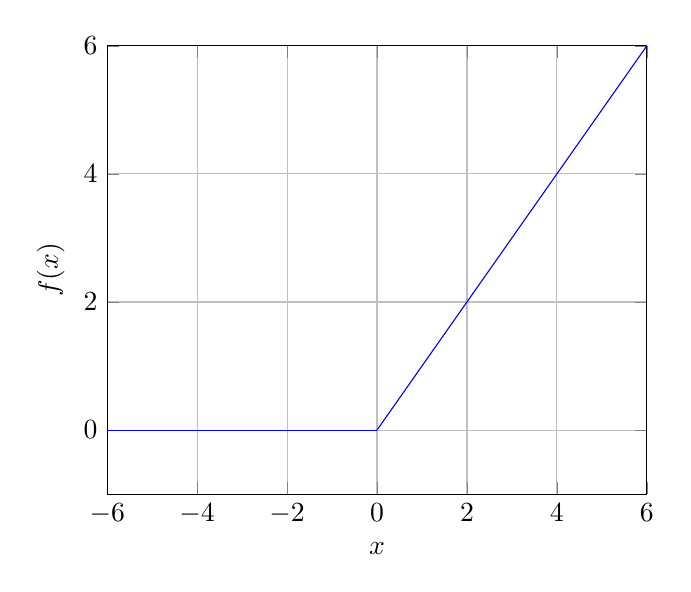
\begin{tikzpicture}
\begin{axis}[
xlabel={$x$},
ylabel={$f(x)$},
clip=false,
grid=major,
xmin=-6, xmax=6,
ymin=-1, ymax=6,
domain=-6:6
]
 \addplot+[mark=none,smooth, blue,domain=-6:0] {0};
  \addplot+[mark=none,smooth, blue,domain=0:6] {x};
\end{axis}
\end{tikzpicture}
\caption{ReLU function}
\label{fig:relu}
\end{figure}

Pooling Layers are used to perform a downsampling operation along the spatial dimensions (width, height). After all, we must reduce an input image dimensions to produce an output of expected dimensions.  It is common to periodically insert a Pooling layer in-between successive convolutional layers in a ConvNet architecture.

A simple CNN for classification could have the architecture [INPUT - CONV - RELU - POOL - FC]. A similar architecture is shown in the Figure \ref{fig:cnn}.

 For more information about CNNs, please consider the original paper\cite{krizhevsky2012imagenet}. 
 
\begin{figure}[h]
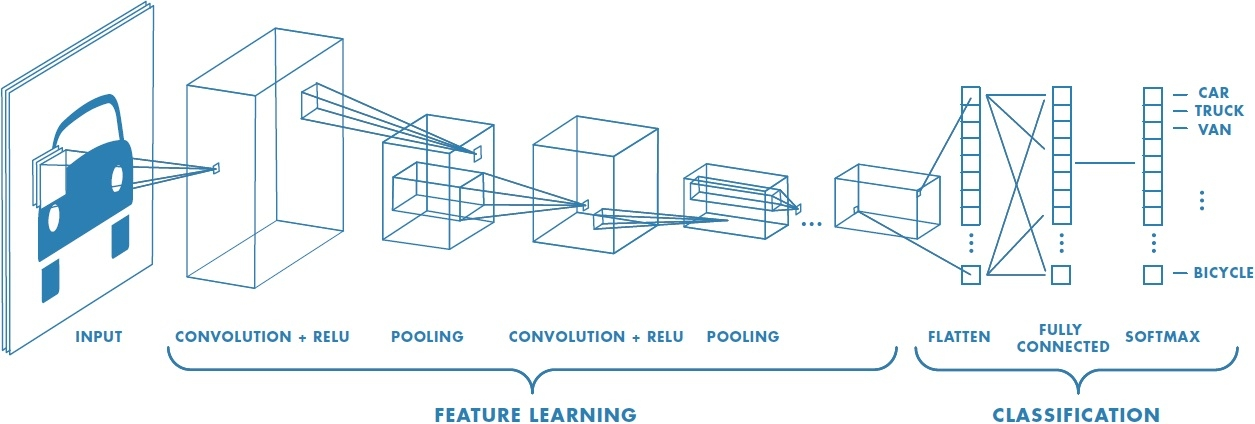
\includegraphics[width=13cm]{cnn}
\caption{A simple deep neural network, image taken from \url{floydhub.com}}
\label{fig:cnn}
\end{figure}

